\section{Observations}
	\subsection{Frequency dependence of Dielectric Constant}
	We connect the probe setup for all these different samples used here. The probe leads (capacitor terminals) are fed to a main unit and an oscilloscope. For every frequency, the variable capacitance $C_4$ and the variable resistance $R_4$ are varies to achieve minimum (almost zero) signal on the oscilloscope, and they are recorded in the following tables. 
	For all these cases,
	\begin{itemize}
		\item $R_3 = 1$ k$\ohm$
		\item $C_2 = 1000$ pF
	\end{itemize}

	\subsubsection{BaTiO$_3$}

		\begin{itemize}
			\item Permittivity of Space $(\epsilon_0) = 8.85\times10^{-3}$ pF mm$^{-1}$
			\item Thickness $(t) = 1.6$ mm
			\item Diameter = $10.56$ mm
			\item Area $(A) = 87.58$ mm$^2$
			\item $C_0 =\frac{\epsilon A}{t} = 0.484$ pF
		\end{itemize}

		\begin{table}[H]
    \centering
    \begin{tabular}{|c|c|c|c|c|c|c|}
    \hline
    $f$ (kHz) & $C_4$ (pF) & $R_4$ (k$\Omega$) & $C_1$ (pF) & $R_1$ ($\Omega$) & $\epsilon$ & $\delta$ \\ \hline
    10 & 550 & 0.908 & 908 & 550 & 1874.3 & 0.0313 \\ \hline
    15 & 400 & 0.900 & 900 & 400 & 1857.8 & 0.0338 \\ \hline
    20 & 300 & 0.896 & 896 & 300 & 1849.6 & 0.0337 \\ \hline
    25 & 250 & 0.894 & 894 & 250 & 1845.4 & 0.0350 \\ \hline
    30 & 200 & 0.890 & 890 & 200 & 1837.2 & 0.0334 \\ \hline
    35 & 150 & 0.888 & 888 & 150 & 1833.0 & 0.0292 \\ \hline
    40 & 150 & 0.886 & 886 & 150 & 1828.9 & 0.0333 \\ \hline
    45 & 150 & 0.884 & 884 & 150 & 1824.8 & 0.0374 \\ \hline
    50 & 100 & 0.882 & 882 & 100 & 1820.7 & 0.0276 \\ \hline
    \end{tabular}
    \caption{Measured values of $\epsilon$ and $\delta$ for different frequencies for BaTiO$_3$ sample}
    \label{tab:a}
\end{table}

		Note that for small values we approximate $\tan \delta = \delta$. The error in $\epsilon$ can be calculated from Eq. 4 as (assuming $\Delta C_0 = \Delta R_3 = \Delta C_2 = 0$),
		\begin{align}
			\frac{\Delta \epsilon}{\epsilon} = \frac{\Delta C_1}{ C_1} = \frac{\Delta R_4}{ R_4}
		\end{align}

		where $\Delta R_4$ is the least count in the measurement of $R_4$, which is $0.002$ k$\Omega$.

		Similarly the error in $\delta$ can be calculated from Eq. 6 as
		\begin{align}
			\frac{\Delta \delta}{\delta} &= \sqrt{\left(\frac{\Delta C_1}{C_1}\right)^2 + \left(\frac{\Delta R_1}{R_1}\right)^2 + \left(\frac{\Delta f}{f}\right)^2}\\
			&= \sqrt{\left(\frac{\Delta R_4}{R_4}\right)^2 + \left(\frac{\Delta C_4}{C_4}\right)^2 + \left(\frac{\Delta f}{f}\right)^2}
		\end{align}

		where $\Delta C_4 = 50$ pF and $\Delta f = 1$ kHz.

		\begin{figure}[H]
			% \ContinuedFloat
			% \bigskip
			\begin{subfigure}{\linewidth}
			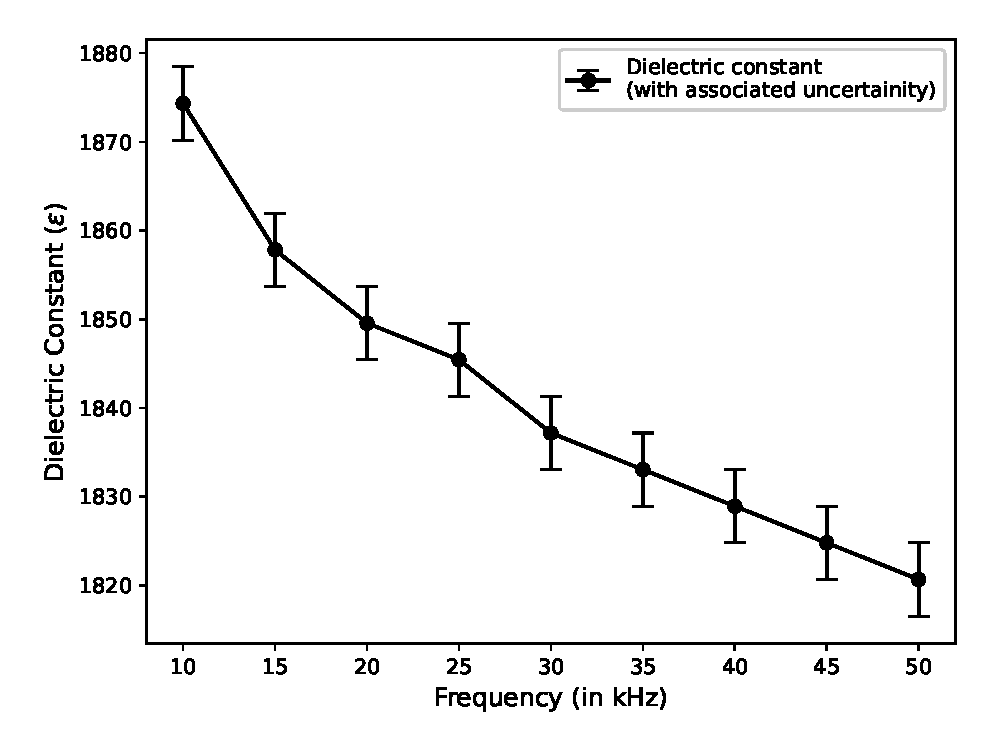
\includegraphics[width=1\textwidth]{images/batio3_e.eps}
			\caption{Dielectric constant vs frequency}
			\end{subfigure}
			
			% \bigskip
			\begin{subfigure}{\linewidth}
			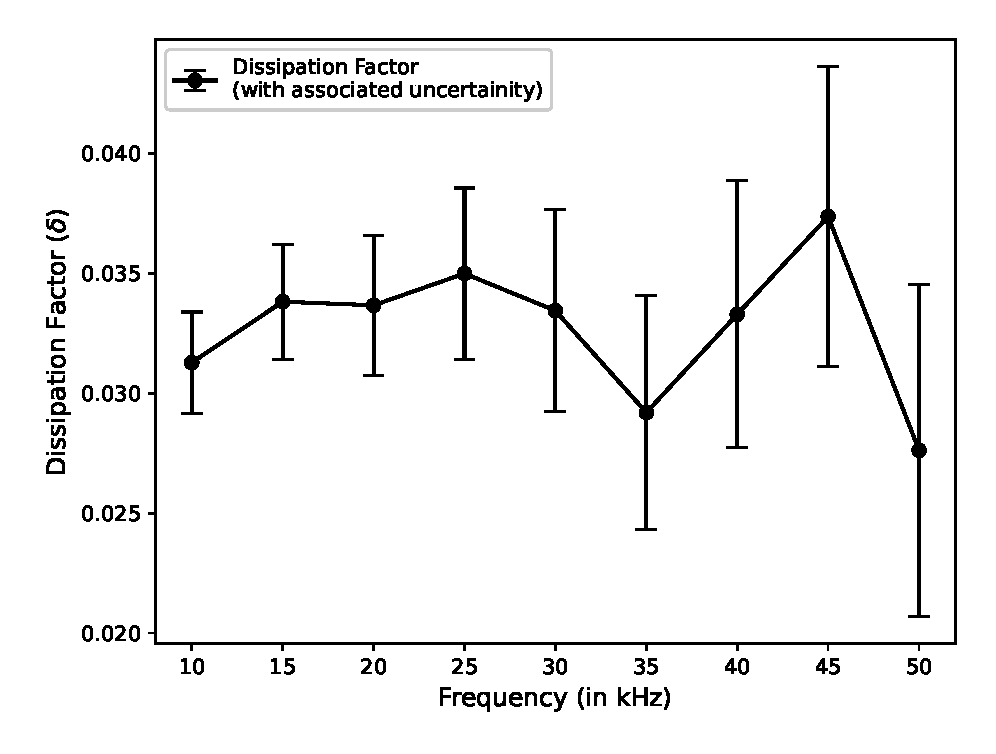
\includegraphics[width=1\textwidth]{images/batio3_d.eps}
			\caption{Dissipation factor vs frequency}
			\label{g1b}
			\end{subfigure}

			\caption{Frequency dependent plots for BaTiO$_3$}
			\label{g1}
		\end{figure}

	These observations show a
	noticeable decline in the dielectric constant as the
	frequency increases. This behavior is expected, as
	at higher frequencies, the polarization response of
	BaTiO$_3$ becomes insufficient to keep up with the
	swiftly varying electric field, resulting in a reduced
	effective dielectric constant.

	The curve for dissipation/loss factor however demonstrates a
	non-monotonic trend. This could be due to the multiple energy dissipation mechanisms, such dipolar relaxation and domain wall dynamics, contributing differently across the frequency spectrum. It is also to be noted that due to the low precision in the variation of $C_4$, the error bars associated with the dissipation factor are too large to make any proper remarks.

	\subsubsection{Multi-layer Ceramic Capacitor (MLCC)}

	\noindent Similarly, we now study the variation of dielectric constant with frequency for a standard MLCC. Here, the DC capacitance of the capacitor was measured to be, $C_0 = 473.1$ pF.

	\begin{table}[H]
    \centering
    \begin{tabular}{|c|c|c|c|c|c|c|}
    \hline
    $f$ (kHz) & $C_4$ (pF) & $R_4$ (k$\Omega$) & $C_1$ (pF) & $R_1$ ($\Omega$) & $\epsilon$ & $\delta$ \\ \hline
    10 & 600 & 0.590 & 590 & 600 & 1.247 & 0.0222 \\ \hline
    15 & 450 & 0.589 & 589 & 450 & 1.245 & 0.0249 \\ \hline
    20 & 350 & 0.587 & 587 & 350 & 1.241 & 0.0257 \\ \hline
    25 & 250 & 0.587 & 587 & 250 & 1.241 & 0.0230 \\ \hline
    30 & 250 & 0.586 & 586 & 250 & 1.239 & 0.0275 \\ \hline
    35 & 200 & 0.586 & 586 & 200 & 1.239 & 0.0257 \\ \hline
    40 & 200 & 0.586 & 586 & 200 & 1.239 & 0.0294 \\ \hline
    45 & 150 & 0.584 & 584 & 150 & 1.234 & 0.0247 \\ \hline
    50 & 150 & 0.584 & 584 & 150 & 1.234 & 0.0274 \\ \hline
    \end{tabular}
    \caption{Measured values of $\epsilon$ for a standard MLCC}
    \label{tab:b}
\end{table}
	\begin{figure}[H]
		\centering
		\label{graph:3}
		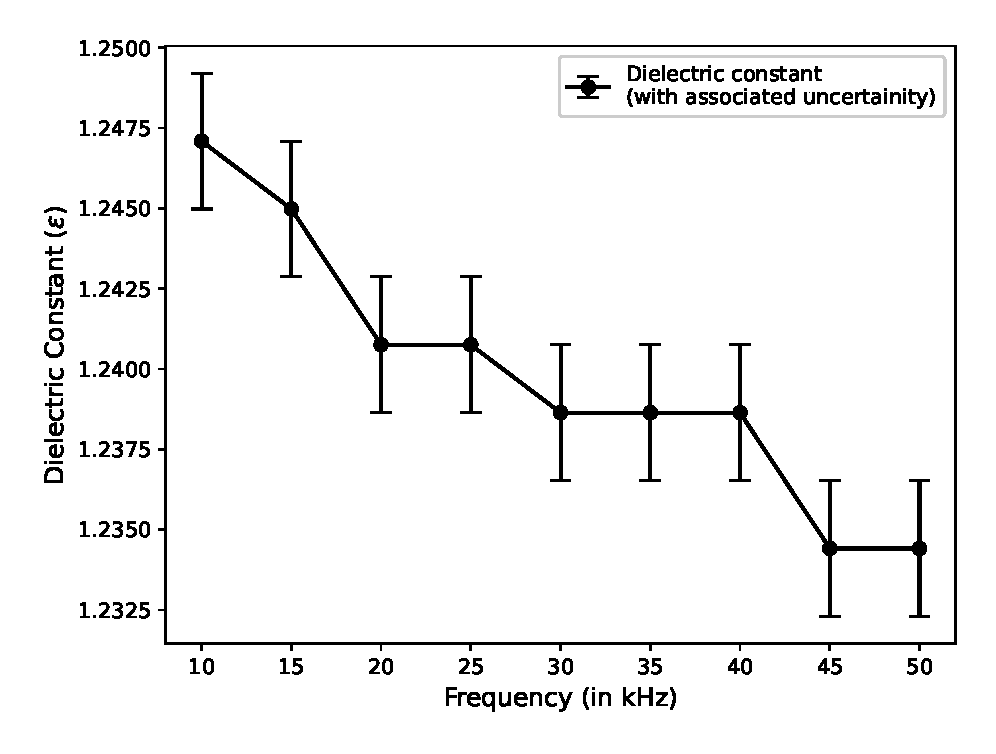
\includegraphics[width=1\columnwidth]{images/mlcc_e.eps}
		\caption{Dielectric constant ($\epsilon$) vs frequency graph for MLCC}
	\end{figure}
	The above plot shows the general trend in the in the variation of $\epsilon$ with frequency, which is decreasing as expected. The plateaus might indicate a shift in the dominant polarization mechanism, leading
	to a brief period of capacitance stability before it
	begins to decline further.

	We have not plotted the variation in the dissipation factor as the values obtained showed no general trend along with the associated error bars being of the order of the variations (see Fig. \ref{g1b}). 

	\subsubsection{Disc Ceramic Capacitor (DCC)}
	% \vspace{-1em}
	\noindent We now study the variation of dielectric constant with frequency for a standard DCC. Here, the standard capacitance of the capacitor was measured to be, $C_0 = 423.3$ pF. 
	% \vspace{-2em}
	\begin{table}[H]
    \centering
    \begin{tabular}{|c|c|c|c|c|c|c|}
    \hline
    $f$ (kHz) & $C_4$ (pF) & $R_4$ (k$\Omega$) & $C_1$ (pF) & $R_1$ ($\Omega$) & $\epsilon$ & $\delta$ \\ \hline
    10 & 550 & 0.526 & 526 & 550 & 1.243 & 0.0181 \\ \hline
    15 & 400 & 0.524 & 524 & 400 & 1.238 & 0.0197 \\ \hline
    20 & 300 & 0.524 & 524 & 300 & 1.238 & 0.0197 \\ \hline
    25 & 250 & 0.523 & 523 & 250 & 1.236 & 0.0205 \\ \hline
    30 & 200 & 0.522 & 522 & 200 & 1.233 & 0.0196 \\ \hline
    35 & 200 & 0.522 & 522 & 200 & 1.233 & 0.0229 \\ \hline
    40 & 150 & 0.522 & 522 & 150 & 1.233 & 0.0196 \\ \hline
    45 & 150 & 0.521 & 521 & 150 & 1.231 & 0.0220 \\ \hline
    50 & 150 & 0.520 & 520 & 150 & 1.228 & 0.0244 \\ \hline
    \end{tabular}
    \caption{Measured values of $\epsilon$ for a standard DCC}
    \label{tab:c}
\end{table}
	% \vspace{-5em}
	\begin{figure}[H]
		\centering
		\label{graph:4}
		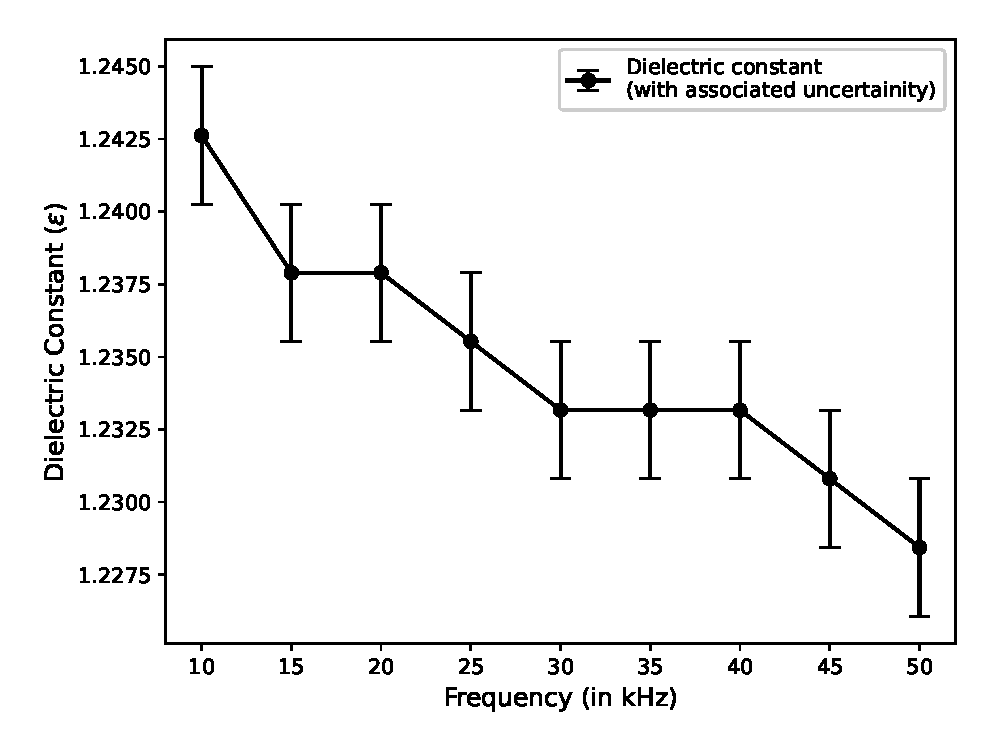
\includegraphics[width=1\columnwidth]{images/disc_e.eps}
		\caption{Dielectric constant ($\epsilon$) vs frequency graph for DCC}
	\end{figure}
	As expected, the above plot shows the general decreasing trend in the in the variation of $\epsilon$ with frequency, as explained in the previous part for MLCC.

	Again, we have not plotted the variation in the dissipation factor as the values obtained showed no general trend along with the associated error bars being of the order of the variations (see Fig. \ref{g1b}). 

\subsection{Temperature dependence of dielectric constant at different frequencies using BaTiO$_3$}

In the second part of the experiment, we obtained
data to study the variation of dielectric constant
of BaTiO$_3$ with temperature for various frequencies.

For this setup, the probe arrangement is
mounted in suitable stand as before, which also hold the sample plate and RTD (Resistance Temperature Detector) sensor. The RTD is mounted in the sample plates such that it is just below the sample, separated by a very thin sheet of mica. This ensures the correct measurement of sample temperature. This stand also
serves as a lid of the oven. The leads are provided for the connection to RTD and capacitance meter. 

After setting the temperature in the oven, we wait around 10 minutes for the temperature to stabilise before taking any readings.

	\begin{table}[H]
    \centering
    \begin{tabular}{|c|c|c|c|c|c|}
    \hline
    T ($^\circ$C) & $C_4$ (pF) & $R_4$ (k$\Omega$) & $C_1$ (pF) & $R_1$ ($\Omega$) & $\epsilon$ \\ \hline
    50 & 550 & 931 & 931 & 550 & 1921.80 \\ \hline
    60 & 600 & 946 & 946 & 600 & 1952.77 \\ \hline
    70 & 550 & 982 & 982 & 550 & 2027.08 \\ \hline
    80 & 700 & 1020 & 1020 & 700 & 2105.52 \\ \hline
    90 & 750 & 1084 & 1084 & 750 & 2237.63 \\ \hline
    100 & 900 & 1156 & 1156 & 900 & 2386.26 \\ \hline
    110 & 850 & 1282 & 1282 & 850 & 2646.35 \\ \hline
    120 & 900 & 1505 & 1505 & 900 & 3106.67 \\ \hline
    125 & 950 & 1658 & 1658 & 950 & 3422.50 \\ \hline
    130 & 800 & 1804 & 1804 & 800 & 3723.88 \\ \hline
    135 & 850 & 1922 & 1922 & 850 & 3967.46 \\ \hline
    140 & 700 & 1867 & 1867 & 700 & 3853.93 \\ \hline
    145 & 650 & 1742 & 1742 & 650 & 3595.90 \\ \hline
    150 & 550 & 1600 & 1600 & 550 & 3302.78 \\ \hline
    160 & 600 & 1369 & 1369 & 600 & 2825.94 \\ \hline
    170 & 700 & 1216 & 1216 & 700 & 2510.11 \\ \hline
    \end{tabular}
    \caption{Dielectric constant as a function
    of temperature for the frequency 10 kHz}
    \label{tab:f1}
\end{table} 
	\begin{table}[H]
    \centering
    \begin{tabular}{|c|c|c|c|c|c|}
    \hline
    T ($^\circ$C) & $C_4$ (pF) & $R_4$ (k$\Omega$) & $C_1$ (pF) & $R_1$ ($\Omega$) & $\epsilon$ \\ \hline
    50 & 250 & 914 & 914 & 250 & 1886.711 \\ \hline
    60 & 250 & 932 & 932 & 250 & 1923.867 \\ \hline
    70 & 250 & 963 & 963 & 250 & 1987.858 \\ \hline
    80 & 350 & 1002 & 1002 & 350 & 2068.363 \\ \hline
    90 & 350 & 1059 & 1059 & 350 & 2186.025 \\ \hline
    100 & 300 & 1130 & 1130 & 300 & 2332.585 \\ \hline
    110 & 400 & 1246 & 1246 & 400 & 2572.036 \\ \hline
    120 & 450 & 1450 & 1450 & 450 & 2993.14 \\ \hline
    125 & 400 & 1574 & 1574 & 400 & 3249.105 \\ \hline
    130 & 400 & 1706 & 1706 & 400 & 3521.584 \\ \hline
    135 & 400 & 1816 & 1816 & 400 & 3748.65 \\ \hline
    140 & 350 & 1764 & 1764 & 350 & 3641.31 \\ \hline
    145 & 400 & 1656 & 1656 & 400 & 3418.373 \\ \hline
    150 & 350 & 1548 & 1548 & 350 & 3195.435 \\ \hline
    160 & 350 & 1366 & 1340 & 350 & 2766.075 \\ \hline
    170 & 350 & 1190 & 1190 & 350 & 2456.439 \\ \hline
    \end{tabular}
    \caption{Dielectric constant as a function
    of temperature for the frequency 25 kHz}
    \label{tab:f2}
\end{table}
	\begin{table}[H]
    \centering
    \begin{tabular}{|c|c|c|c|c|c|}
    \hline
    T ($^\circ$C) & $C_4$ (pF) & $R_4$ (k$\Omega$) & $C_1$ (pF) & $R_1$ ($\Omega$) & $\epsilon$  \\ \hline
    50 & 200 & 908 & 908 & 200 & 1874.325 \\ \hline
    60 & 200 & 928 & 928 & 200 & 1915.61 \\ \hline
    70 & 200 & 954 & 954 & 200 & 1969.28 \\ \hline
    80 & 200 & 998 & 998 & 200 & 2060.106 \\ \hline
    90 & 300 & 1048 & 1048 & 300 & 2163.318 \\ \hline
    100 & 300 & 1120 & 1120 & 300 & 2311.943 \\ \hline
    110 & 300 & 1234 & 1234 & 300 & 2547.266 \\ \hline
    120 & 300 & 1431 & 1431 & 300 & 2953.92 \\ \hline
    125 & 300 & 1548 & 1548 & 300 & 3195.435 \\ \hline
    130 & 300 & 1673 & 1673 & 300 & 3453.465 \\ \hline
    135 & 300 & 1768 & 1768 & 300 & 3649.567 \\ \hline
    140 & 300 & 1738 & 1738 & 300 & 3587.64 \\ \hline
    145 & 250 & 1620 & 1620 & 250 & 3344.06 \\ \hline
    150 & 300 & 1521 & 1521 & 300 & 3139.701 \\ \hline
    160 & 300 & 1296 & 1296 & 300 & 2675.248 \\ \hline
    170 & 300 & 1178 & 1178 & 300 & 2431.669 \\ \hline
    \end{tabular}
    \caption{Dielectric constant as a function
    of temperature for the frequency 35 kHz}
    \label{tab:f3}
\end{table}
	\begin{table}[H]
    \centering
    \begin{tabular}{|c|c|c|c|c|c|}
    \hline
    T ($^\circ$C) & $C_4$ (pF) & $R_4$ (k$\Omega$) & $C_1$ (pF) & $R_1$ ($\Omega$) & $\epsilon$\\ \hline
    50 & 150 & 902 & 902 & 150 & 1861.94 \\ \hline
60 & 150 & 922 & 922 & 150 & 1903.224 \\ \hline
70 & 150 & 946 & 946 & 150 & 1952.766 \\ \hline
80 & 150 & 990 & 990 & 150 & 2043.592 \\ \hline
90 & 250 & 1036 & 1036 & 250 & 2138.547 \\ \hline
100 & 250 & 1116 & 1116 & 250 & 2303.686 \\ \hline
110 & 300 & 1216 & 1216 & 300 & 2510.109 \\ \hline
120 & 250 & 1406 & 1406 & 250 & 2902.314 \\ \hline
125 & 300 & 1528 & 1528 & 300 & 3154.151 \\ \hline
130 & 200 & 1632 & 1632 & 200 & 3368.831 \\ \hline
135 & 200 & 1744 & 1744 & 200 & 3600.025 \\ \hline
140 & 200 & 1706 & 1706 & 200 & 3521.584 \\ \hline
145 & 200 & 1589 & 1589 & 200 & 3280.069 \\ \hline
150 & 250 & 1500 & 1500 & 250 & 3096.352 \\ \hline
160 & 200 & 1280 & 1280 & 200 & 2642.22 \\ \hline
170 & 250 & 1160 & 1160 & 250 & 2394.512 \\ \hline
    \end{tabular}
    \caption{Dielectric constant as a function
    of temperature for the frequency 50 kHz}
    \label{tab:f4}
    \end{table}
	\begin{figure*}
		\centering
		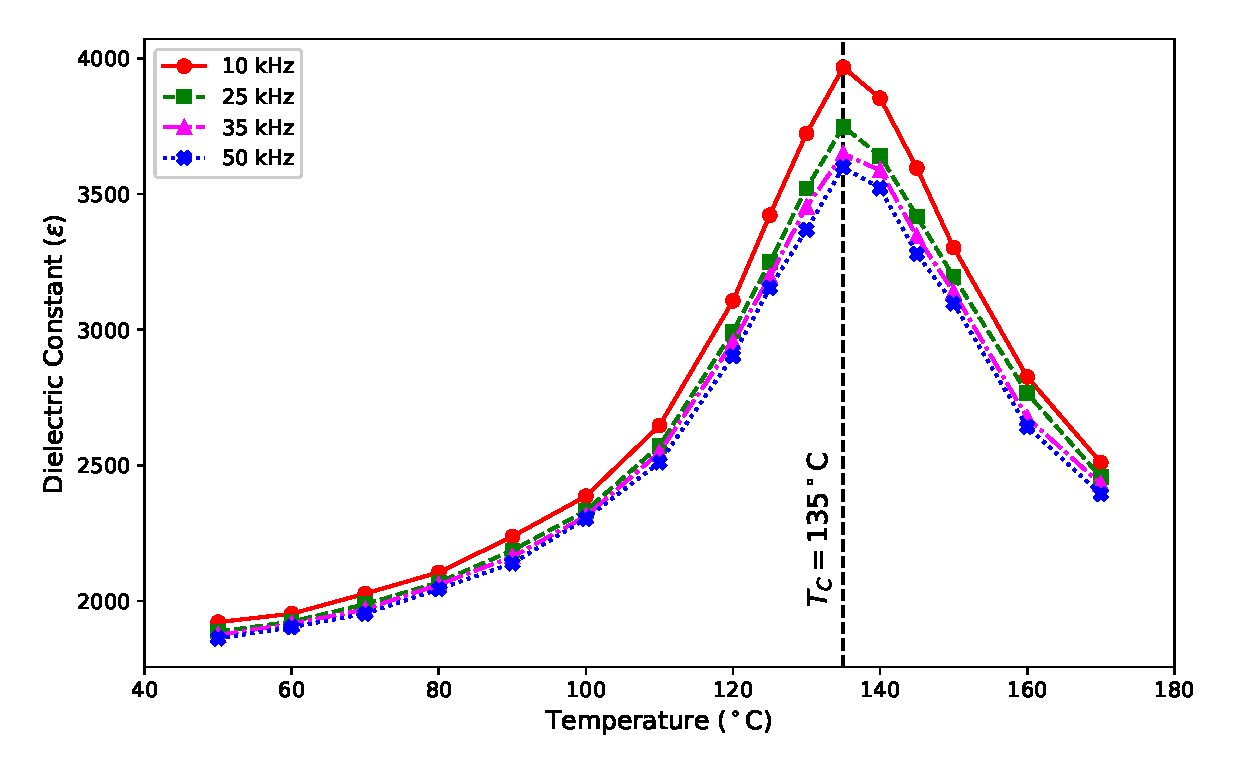
\includegraphics[width=1.5\columnwidth]{images/temp.eps}
		\caption{Variation of Dielectric constant with Temperature T ($^\circ$C) for four different frequencies}
		\label{graph:5}
	\end{figure*}

	Fig. 7 shows the variation in the dielectric constant with temperature, at four different frequencies. The curves are nearly symmetrical, and the dielectric constant peaks at a specific temperature (the Curie temperature). While the magnitude of the dielectric constant increases as the frequency decreases (as explained in the previous sections), the difference is not quite noticable at this scale.
	
	The Curie temperature is found to be around 135 $^\circ$C from the graph. Since we took measurements only at every 5$^\circ$C near $T_C$, the standard deviation associated with the readings must be 5$^\circ$C.  
	
	\subsubsection*{Study of diffuseness parameter at a single frequency}
	\vspace{-1em}

	Diffuseness parameter can be calculated as the slope of $\log(\frac{1}{\epsilon}-\frac{1}{\epsilon_C})$ and $\log(T-T_C)$, for all values above the Curie Temperature. $\epsilon_c$ is the maximum dielectric constant, which is obtained at the Curie temperature. 
	We have plotted the required quantities for all four values of frequencies below.

	\vspace{-5em}

	\begin{figure}[H]
		% \ContinuedFloat
		% \bigskip
		\begin{subfigure}{\linewidth}
		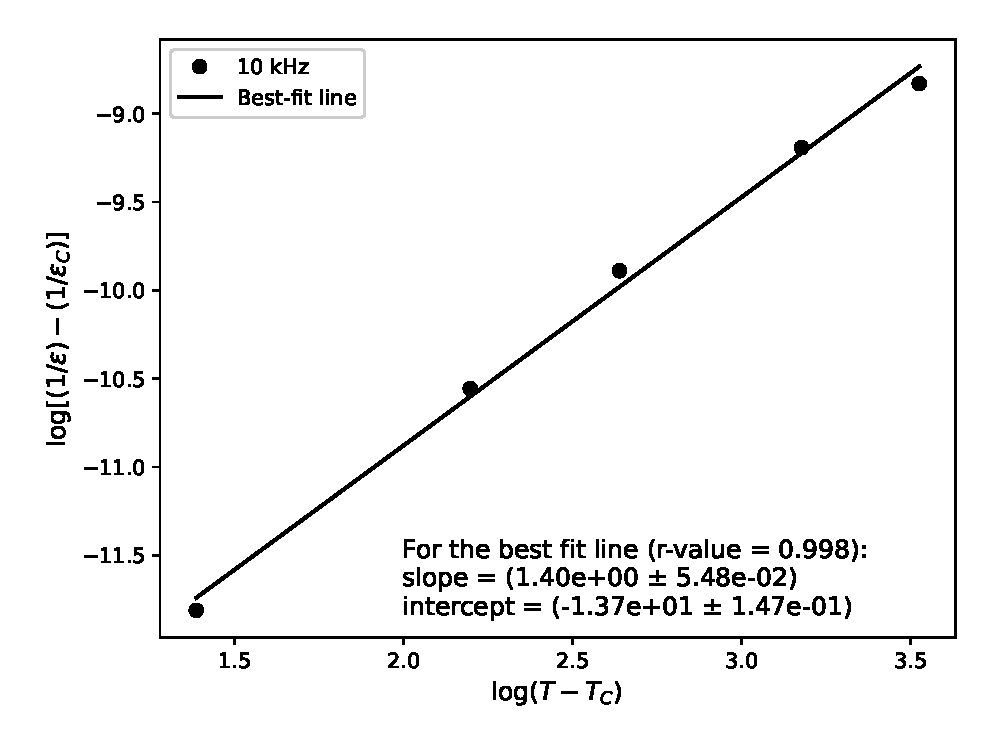
\includegraphics[width=1\textwidth]{images/TC10.eps}
		\caption{10 kHz}
		\end{subfigure}
		
		% \bigskip
		\begin{subfigure}{\linewidth}
		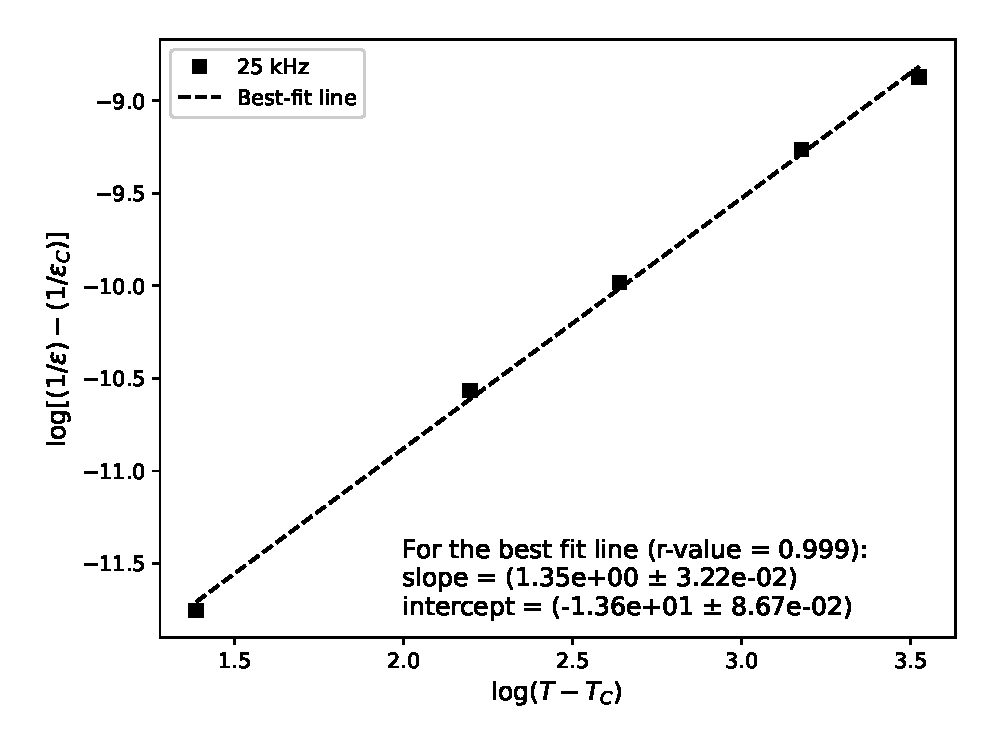
\includegraphics[width=1\textwidth]{images/TC25.eps}
		\caption{25 kHz}
		\end{subfigure}
		
		\begin{subfigure}{\linewidth}
		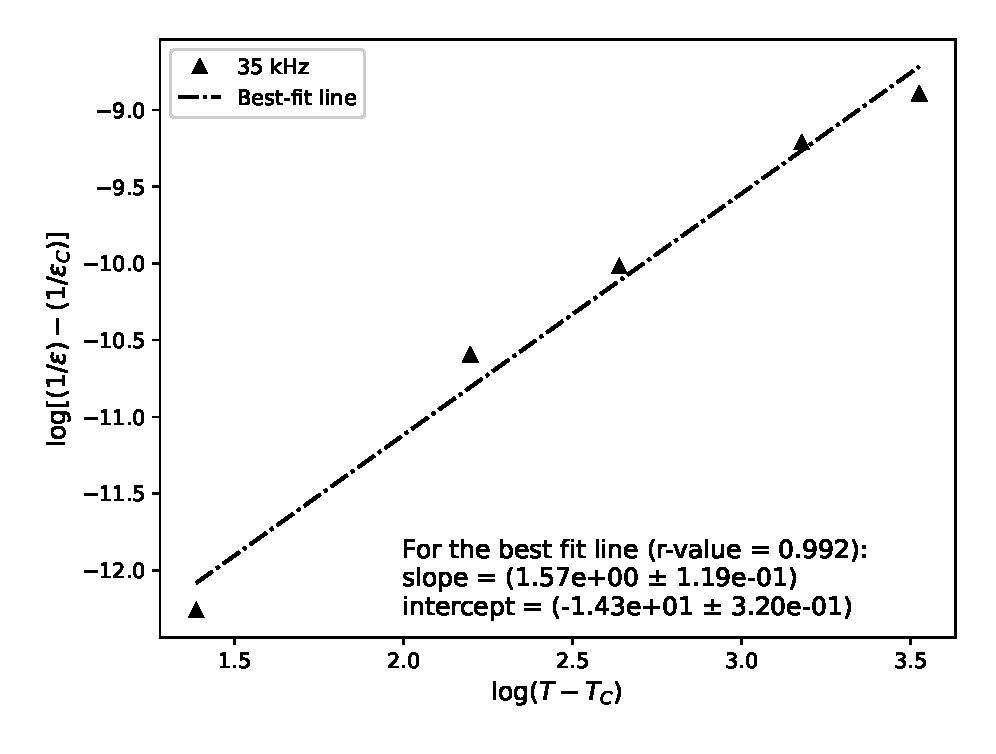
\includegraphics[width=1\textwidth]{images/TC35.eps}
		\caption{35 kHz}
		\end{subfigure}
	\end{figure}

	\begin{figure}[H]
		\ContinuedFloat
		\begin{subfigure}{\linewidth}
		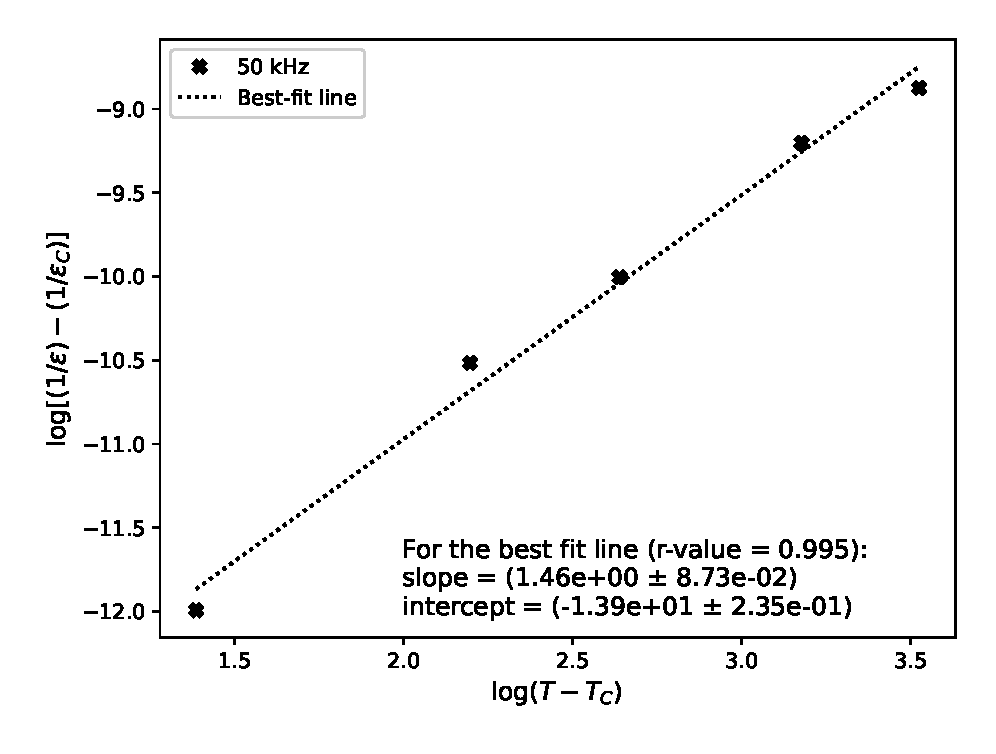
\includegraphics[width=1\textwidth]{images/TC50.eps}
		\caption{50 kHz}
		\end{subfigure}

		\caption{$\log(\frac{1}{\epsilon}-\frac{1}{\epsilon_C})$ vs. $\log(T-T_C)$ at different frequencies}
		\label{final}
	\end{figure}
		
	From the above plots, the average value of $\delta$ can be taken as the slops obtained using linear regression.